\section*{Задача 4.3}
\subsection*{Постановка задачи}
Задана функция $f(x) = e^{2x} - 1$, определенная на отрезке $[-1, 1]$. Требуется разложить функцию в рял Тейлора в окрестности нуля с точностью $\varepsilon$ и произвести экономизацию полученного степенного ряда.

\subsection*{Теоретический материал}
Суть метода экономизации степенного ряда заключается в следующем:

\begin{enumerate}
	\item Берем отрезок ряда Тейлора $P_m(x) = \sum\limits_{k = 0}^m a_kx_k$, аппроксимирующий функцию $f(x)$ с точностью $\varepsilon_0 < \varepsilon$.
	\item Выражая $x^m$ с помощью многочлена Чебышева, заменяем $x^m$ в разложении Тейлора на $-2^{1 - m}(b_0 + b_1x + \dots + b_{m - 1} x^{m-1}) + 2^{1 - m}T_m(x)$ до тех пор, пока величина погрешности не превысит заданного значения.
\end{enumerate}

\subsection*{Решение}
Запишем разложение функции $f(x) = e^{2x} - 1$ в ряд Тейлора:
\[
	f(x) = e^{2x} - 1 = \sum\limits_{n = 1}^\infty \dfrac{2^nx^n}{n!}
\]

\begin{enumerate}
	\item Определим функцию, вычисляющую $a_k$ коэффициент разложения ряда Тейлора и функцию, вычисляющую значение ряда в данной точке.
	\item Найдем число $n$ - длину ряда, вычисляющего значение функции на заданном отрезке с необходимой точностью с помощью оценки сверху для остаточного члена разложения в форме Лагранжа: $max(r_n(x)) = \dfrac{f^{(n+1)}(\xi)x^{n+1}}{(n+1)!} \leq \dfrac{2^{n+1}}{(n+1)!} \leq \varepsilon$.
	\item Для первого слагаемого замены при экономизации воспользуемся готовыми формулами.
	\item Параллельно будем строить графики получившихся замен до тех пор, пока не достигнем максимально допустимой точности.
\end{enumerate}

Для реализации процесса экономизации степенного ряда воспользуемся встроенными средствами библиотеки NumPy для работы с многочленами - numpy.polynomial.

\newpage
\subsection*{Анализ результатов}
Для того, чтобы достичь необходимой точности ($\varepsilon = 10^{-8}$) необходимо взять 16 членов ряда Тейлора.

Проводя экономизацию ряда с 15 до 11 степени удалось сохранить необходимую точность:
\begin{figure}[h!]
	\centering                                                                                            
	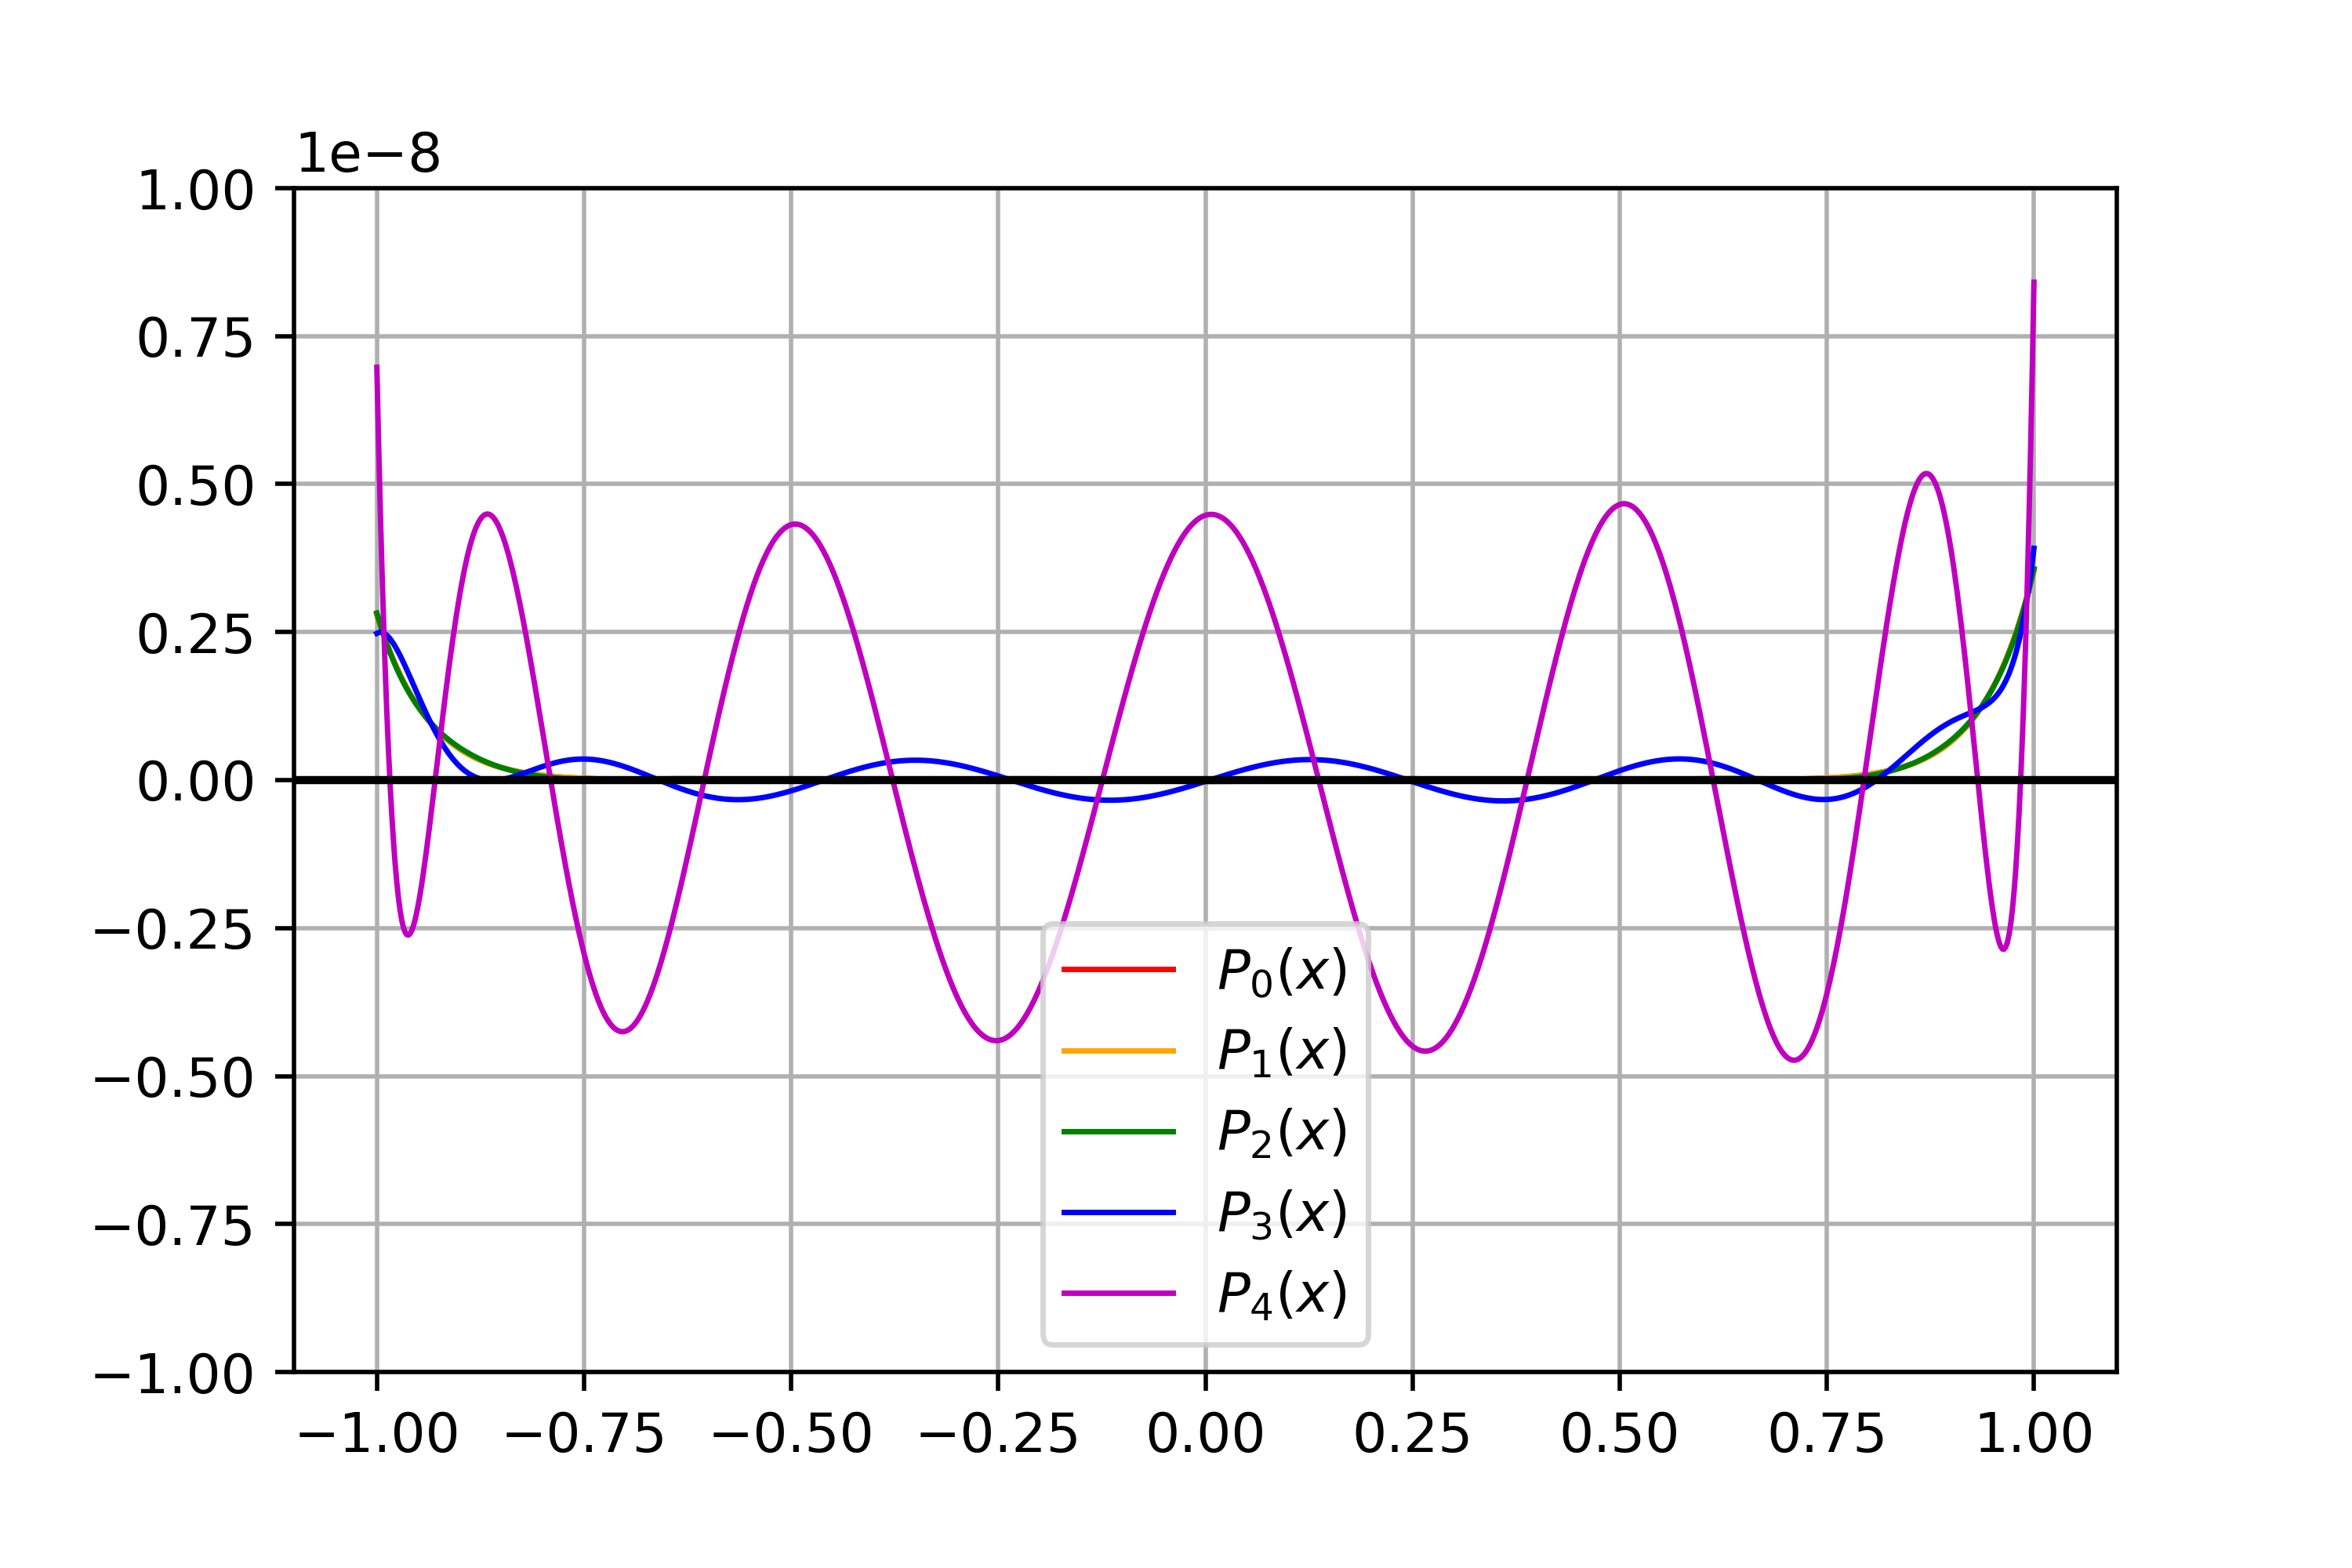
\includegraphics[height=8cm]{images/plot_4.3_err.png}
	\caption{Погрешность ряда на каждом этапе экономизации. $P_0(x)$ - до экономизации. $P_4(x)$  - после завершения процесса}
\end{figure}

График ряда после экономизации:

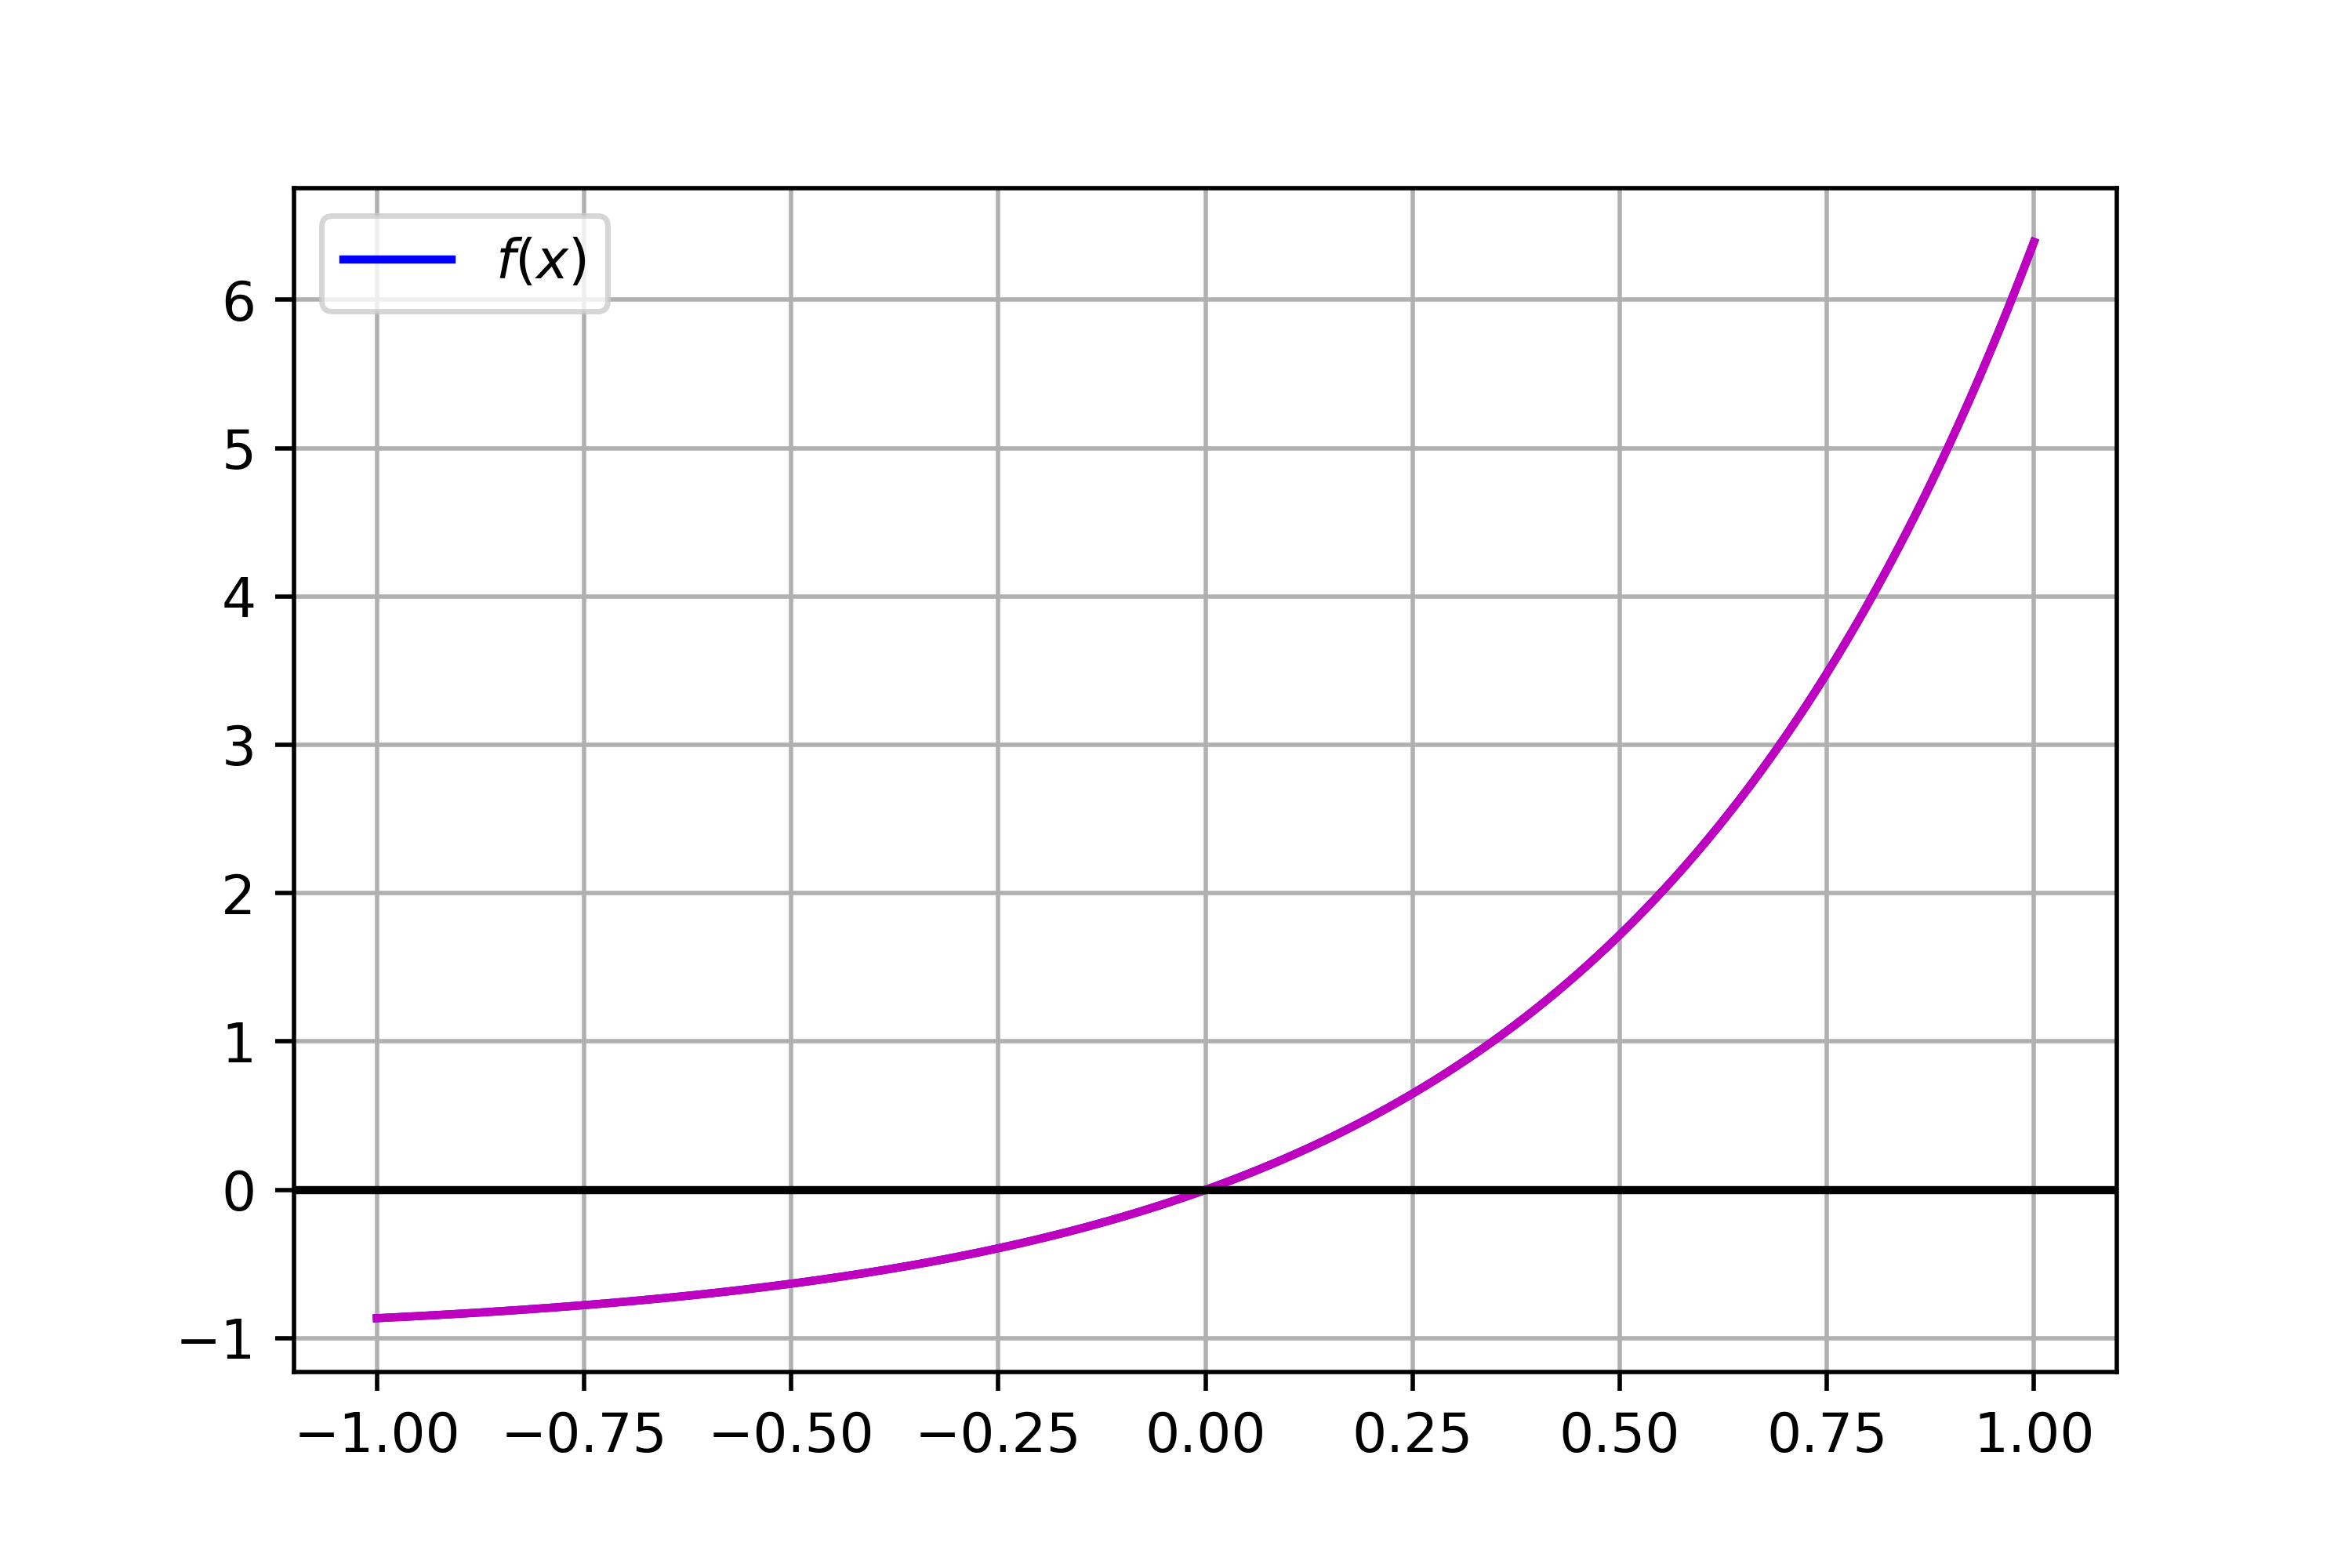
\includegraphics[height=9.5cm]{images/plot_4.3_func.png}

\textbf{Вывод}{
	Увеличение количества членов ряда Тейлора приводит к скачкообразному снижению погрешности и слишком большим степеням многочлена. Как можно видеть, на графике погрешностей до экономизации погрешность избыточно низкая. Экономизация степенного ряда позволяет значительно снизить степень многочлена, сохранив при этом допустимую точность на отрезке.
}
\subsection*{Код программы}
\begin{lstlisting}
import numpy as np
import matplotlib.pyplot as plt
import numpy.polynomial as plnm

f = lambda x: np.exp(2*x) - 1
def Taylor(n):
    power, fact = 1, 1
    while n:
        power, fact = power*2, fact*n
        n -= 1
    return power/fact

def get_n(eps: np.float64) -> int:
    n = 1
    power, fact = 1, 1
    while power/fact >= eps:
        power, fact = power*2, fact*n
        n += 1
    return n-1

def Cheb2Poly(n):
    arr = [0]*n + [1]
    cheb = plnm.chebyshev.Chebyshev(arr)
    poly = plnm.Polynomial(plnm.chebyshev.cheb2poly(cheb.coef))
    return poly

def Economise(P):
    tmpCheb = Cheb2Poly(P.degree())
    PRes = P.cutdeg(P.degree()-1) - P.coef[-1]/(tmpCheb.coef[-1]) * tmpCheb.cutdeg(P.degree()-1)
    return PRes

eps = 1e-8
n = get_n(eps) - 1
a = [Taylor(i) for i in range(1, n+1)]
P0 = plnm.Polynomial([0] + a)
P = [P0]
print(P0.degree(), n)
for i in range(4):
    P.append(Economise(P[-1]))

\end{lstlisting}